\chapter{Record Kstack}
Tato kapitola se bude zabývat modifikací, která dodává uživateli přímější způsob, jak zapínat trasování zásobníku kernelu přes GUI KernelSharku. Modifikace je přímá a velmi jednoduchá, kapitola je tak krátká.

\section{Cíl}
Dát KernelSharku GUI prvek, kterým se zapne/vypne trasování zásobníku kernelu při trasování přes Record okénko.

\section{Analýza}
Jelikož chceme rozšířit GUI, dává smysl se porozhlédnout v kódu KernelSharku po GUI kódu pro Record okno. Jeho kód se nachází v souborech KsCaptureDialog.hpp/cpp - zde tedy budeme modifikovat.

\subsection{Návrh}
Modifikace bude nejspíše malá, proto nemá smysl vymýšlet složitý návrh. Nicméně si jako návrhové cíle vytyčíme jednoduchost použití, to nám zajistí Qt knihovna, a podobnost kódu modifikace s kódem KernelSharku. Tento cíl udělá kód příjemnějším ke čtení v budoucnosti.

\subsection{Implementace}
V hlavičkovém souboru najdeme třídu KsControlCapture, která sdružuje prvky konfigurující zachycování. Do jejích datových členů přidáme zašktávací políčko. V konstruktoru pak toto políčko nezapomeneme iniciovat a nastavit jako nezaškrtnuté jako výchozí stav. Poté najdeme místo, kde se stavy GUI prvků interpretují na konfiguraci zachycení. Zde přibude překlad zašktnutého políčka na přidání argumentu -T k ostatním argumentům pro zachytávací program trace-cmd. Tím bude modifikace dokončena.

\section{Vývojová dokumentace}
Vývojová dokumentace této modifikace slouží k orientaci ve vylepšení.

Modifikace používá značku RECORD KSTACK v ohraničeních změn. Jedinými změněnými soubory jsou \emph{KsCaptureDialog.hpp/cpp} - v těchto souborech je přidáno zaškrtávací políčko do Record okénka KernelSharku, přidána je i inicializace tohoto políčka a význam zaškrtnutí.

Modifikace je pouze rozšíření GUI o políčko a přidání jeho sémantiky zaškrtnutí. Políčko musí být nutně v Record okénku, resp. ve třídě KsCaptureControl, jelikož nikde jinde nemá nastavení vliv.

\section{Uživatelská dokumentace}
Uživatelská dokumentace pojednává hlavně o tom, jak modifikaci instalovat a používat.

\subsection{Uživatel GUI}

Stejně jako u jiných modifikací, pokud již máme instalovaný KernelShark s touto modifikací, není potřeba dělat nic. Jinak se musí KernelShark sestavit pomocí oficiálních instrukcí z kódu s touto modifikací. Tato modifikace nevyžaduje upravený soubor CMakeLists.txt.

Po otevření KernelSharku otevřeme okno Record. Zde najdeme zaškrtávací políčko s popiskem „Enable kernel stack tracing“.
Zaškrtnutím tohoto políčka povolíme trasování zásobníku kernelu. Poté spustíme trasování a otevřeme výsledná data v KernelSharku. Po každé události, vyjímaje události vytvořené KernelSharkem během načítání trasovacích dat, například Couplebreak události, se budou zobrazovat události ftrace/kernel\_stack.

Změny v okénku lze pozorovat na následujícím obrázku \ref{obr01:record-kstack} (obrázek byl zvětšen pomocí AI). Červené obdélníky zvýrazňují místa, kde se Record okno díky modifikaci změnilo. Černé obdélníky schovávají cesty na autorově stroji.

\begin{figure}[p]\centering
    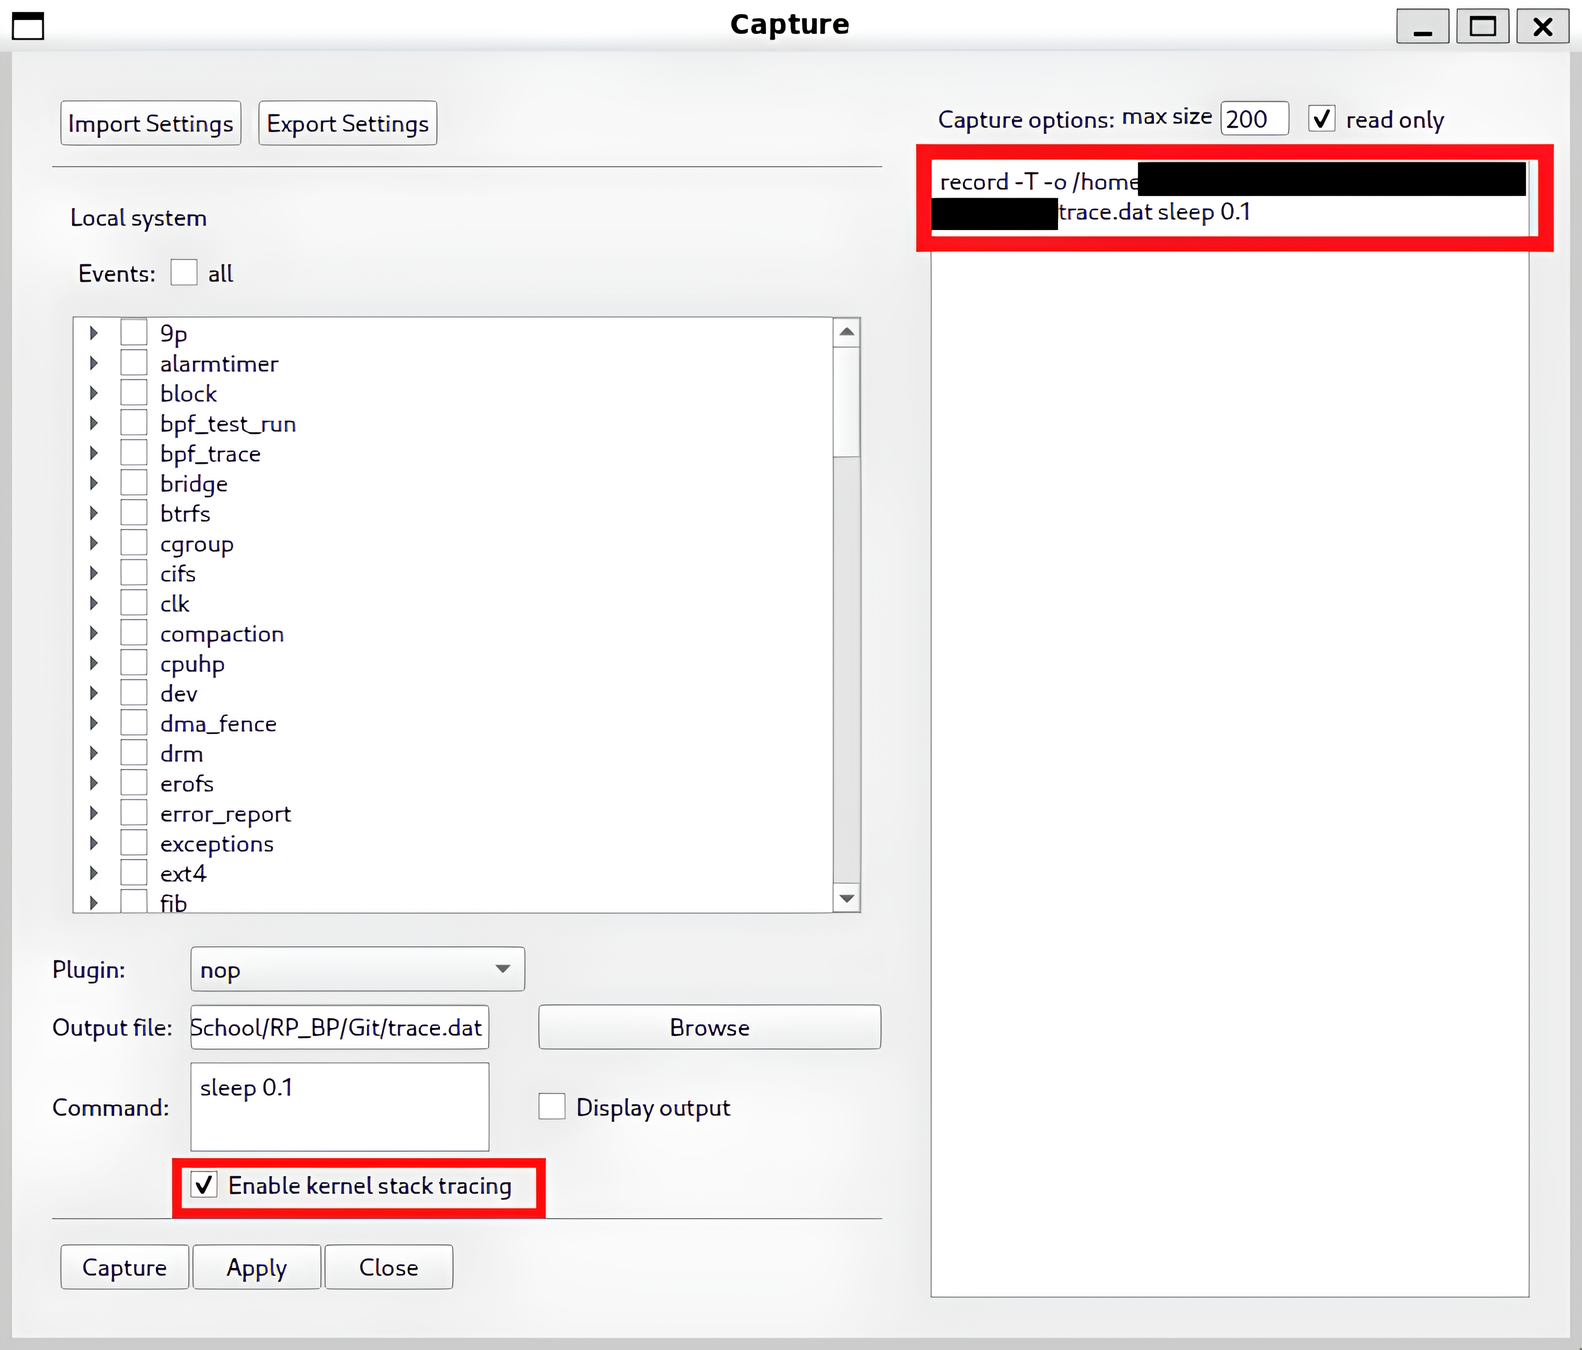
\includegraphics[width=140mm]{img/modif-record-kstack}
    \caption{Zvýraznění změn této modifikace viditelných v GUI}
    \label{obr01:record-kstack}
\end{figure}

\section{Rozšíření}

Ne každá událost může mít zajímavý zásobník. Možnost zachytávat pouze po některých událostech by zde pomohla. Nicméně to je spíše rozšíření pro trace-cmd. KernelShark by mohl umět ignorovat záznamy zásobníku jádra, pokud navazují na nějakou událost, po které nás zásobník nezajímá. Data budou stále v souboru, ale KernelShark by je nenačetl.

\section{Zhodnocení splněných požadavků}
Jediný vlastní požadavek této modifikace bylo přidání zaškrtávacího tlačítka pro jasnější zapínání sběru zásobníků kernelu. Toto bylo splněno přidáním takového tlačítka do Record okénka a připsání interpretace zaškrtnutí jako dodání argumentu trace-cmd.

Obecné požadavky byly splněny také, GUI prvek byl přidán, kód byl rozšířen. Žádná modifikace existujícího chování se neudála. Tlačítko je ve výchozím stavu nezaškrtnuté a lze jej po zaškrtnutí odškrtnout. Tím jsou obecné požadavky splněny.